\section{Task 1: Account Recovery}

\subsection{Most important recommendations for the account recovery process}

\paragraph{General}
\begin{itemize}
	\item Don't store passwords in plain text, but checksums/hashes.
	\item Balance ease of use with challenge.
	\item Regularly revalidate information like current email address, phone numbers etc.
\end{itemize}

\paragraph{Email Authentication}
\begin{itemize}
	\item Focus on recovering the account - not all features
	\item Don't send their old password, but a new, randomly generated password. Or a token.
	\item Notify real account holder over all channels available.
\end{itemize}

\paragraph{Knowledge-Based}
\begin{itemize}
	\item Don't allow easily guessed information.
	\item Plan for cultural differences.
	\item Changes should require at least as much authority as recovery.
\end{itemize}

\paragraph{Social}
\begin{itemize}
	\item Don't spam or otherwise alienate the users social contacts required for information.
\end{itemize}

\paragraph{Multi-Channel Authentication}
\begin{itemize}
	\item Is only useful if independent, so sending a SMS to a phone that is used to recover the account is not helpful.
\end{itemize}

\subsection{Example: dotasource.de}

As test object I used the web site \url{www.dotasource.de}.

This is what the Lost Password page looks like:

\begin{figure}[H]
	\centering
	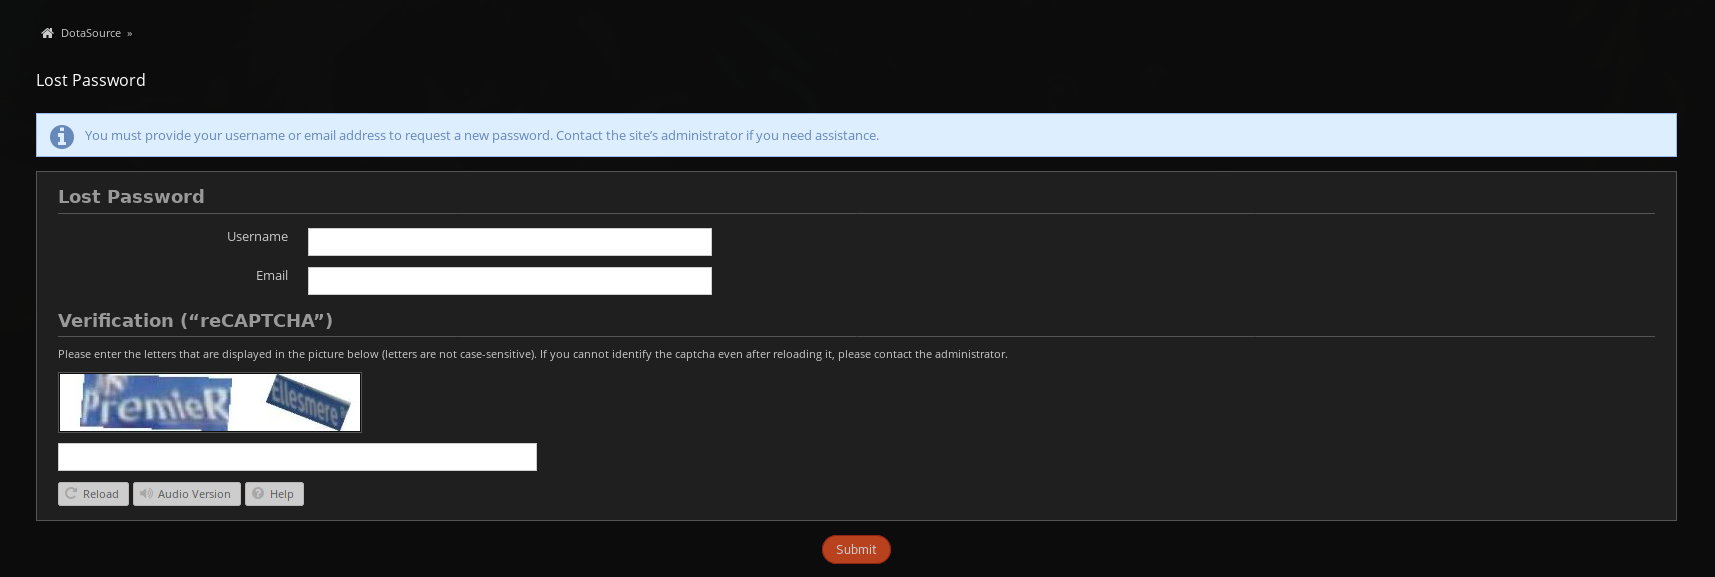
\includegraphics[width=0.8\textwidth]{Assignment0x01/image/recover_1.png}
	\caption{Lost Password} \label{img:recover_1}
\end{figure}

When entered a non-existent username or E-mail address the page responds that the user does not exist or no account with that e-mail is registered.

\begin{figure}[H]
	\centering
	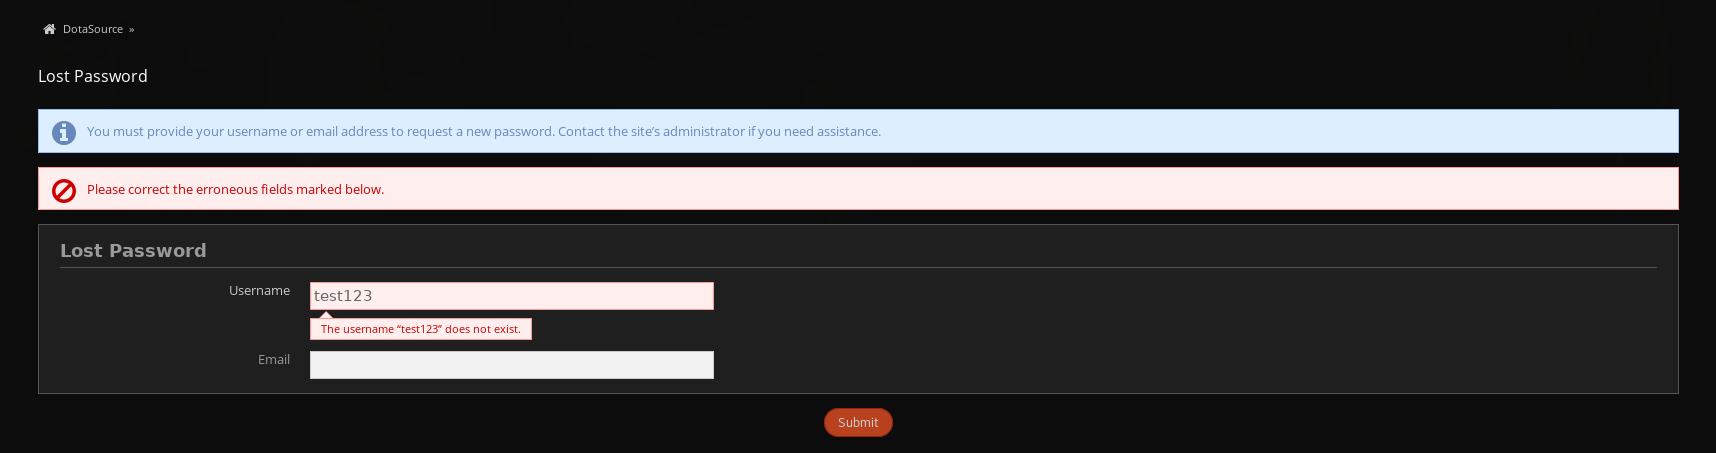
\includegraphics[width=0.8\textwidth]{Assignment0x01/image/recover_2.png}
	\caption{User does not exist} \label{img:recover_2}
\end{figure}

\begin{figure}[H]
	\centering
	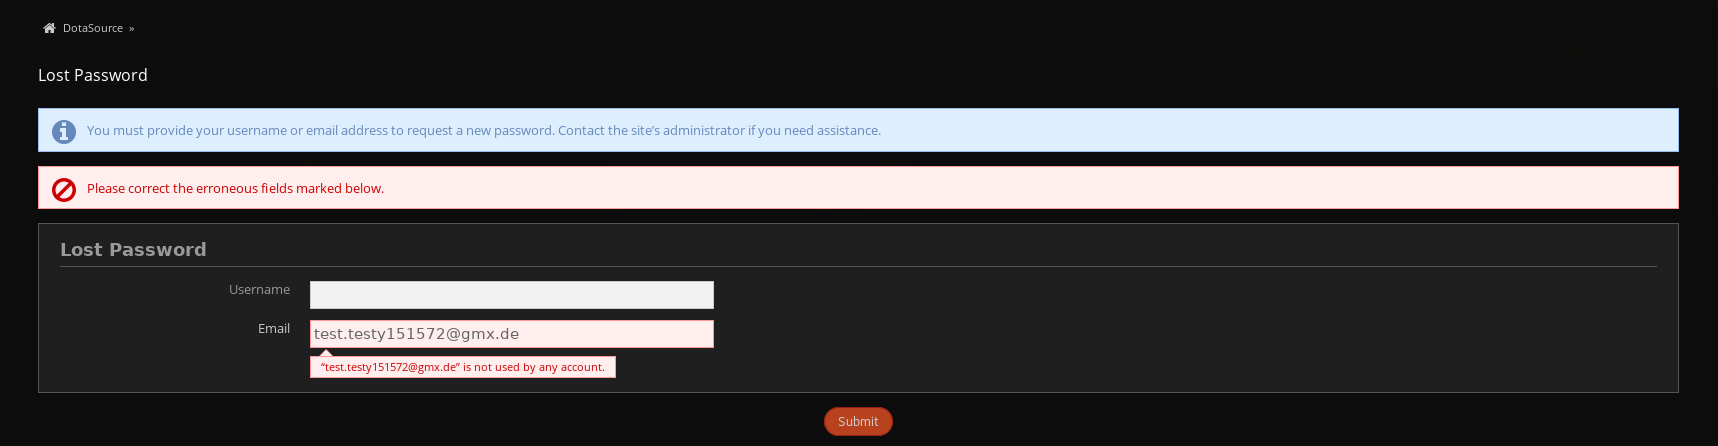
\includegraphics[width=0.8\textwidth]{Assignment0x01/image/recover_3.png}
	\caption{E-mail not used by an account} \label{img:recover_3}
\end{figure}

When entering correct information an email is sent to the account's address, containing a link for recovery.

\begin{figure}[H]
	\centering
	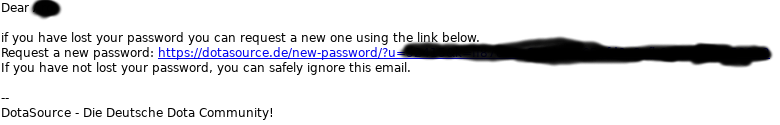
\includegraphics[width=0.8\textwidth]{Assignment0x01/image/email_with_request_link_blacked}
	\caption{Reset Link} \label{img:link_blacked}
\end{figure}

When clicked on the link another email with a new, random generated password in plain text is sent.
Sessions that are still logged in don't lock you out. But for a new login the password is in immediate effect.
To change the password again, you have to login using the given password and visit the account management site.
